\iffalse
\let\negmedspace\undefined
\let\negthickspace\undefined
\documentclass[journal,12pt,twocolumn]{IEEEtran}
\usepackage{cite}
\usepackage{amsmath,amssymb,amsfonts,amsthm}
\usepackage{algorithmic}
\usepackage{graphicx}
\usepackage{textcomp}
\usepackage{xcolor}
\usepackage{txfonts}
\usepackage{listings}
\usepackage{enumitem}
\usepackage{mathtools}
\usepackage{gensymb}
\usepackage{comment}
\usepackage[breaklinks=true]{hyperref}
\usepackage{tkz-euclide}
\usepackage{listings}
\usepackage{gvv}
\def\inputGnumericTable{}
\usepackage[latin1]{inputenc}
\usepackage{color}
\usepackage{array}
\usepackage{longtable}
\usepackage{calc}
\usepackage{multirow}
\usepackage{hhline}
\usepackage{ifthen}
\usepackage{lscape}
\usepackage{circuitikz}

\newtheorem{theorem}{Theorem}[section]
\newtheorem{problem}{Problem}
\newtheorem{proposition}{Proposition}[section]
\newtheorem{lemma}{Lemma}[section]
\newtheorem{corollary}[theorem]{Corollary}
\newtheorem{example}{Example}[section]
\newtheorem{definition}[problem]{Definition}
\newcommand{\BEQA}{\begin{eqnarray}}
\newcommand{\EEQA}{\end{eqnarray}}
\newcommand{\define}{\stackrel{\triangle}{=}}
\theoremstyle{remark}
\newtheorem{rem}{Remark}
\begin{document}

\bibliographystyle{IEEEtran}
\vspace{3cm}

\title{Gate 2021- Instrumentation Engineering}
\author{EE23BTECH11058 - Sindam Ananya$^{*}$% <-this % stops a space
}
\maketitle
\newpage
\bigskip

\renewcommand{\thefigure}{\theenumi}
\renewcommand{\thetable}{\theenumi}

\vspace{3cm}
\textbf{Question 43:} 
Given $y(t) = e^{-3t}u(t) * u(t+3)$, where * denotes convolution operation. The value of $y(t)$ as $t \rightarrow \infty$ is
\hfill{(GATE IN 2021)}\\
\solution
\fi
\begin{align}
y(t) &=  e^{-3t}u(t) * u(t+3)\\
x(t) &\xleftrightarrow{\mathcal{L}} X(s)\\
x(t-t_o) &\xleftrightarrow{\mathcal{L}} e^{-s t_o}X(s)\\
x_1(t) * x_2(t) &\xleftrightarrow{\mathcal{L}} X_1(s)X_2(s)\\
e^{-at}u(t) &\xleftrightarrow{\mathcal{L}} \frac{1}{s + a} \quad \brak{ROC:Re(s)>-a}\\
u(t) &\xleftrightarrow{\mathcal{L}} \frac{1}{s} \quad \brak{ROC:Re(s)>0}\\
u(t+3) &\xleftrightarrow{\mathcal{L}} \frac{e^{3s}}{s} \quad \brak{ROC:Re(s)>0}\\ 
Y(s) &= \brak{\frac{1}{s + 3}}\brak{\frac{e^{3s}}{s}} \quad \brak{ROC:Re(s)>0}
\label{eq:gate202143}
\end{align}
By using Final Value Theorem,
\begin{align}
\lim\limits_{t \to \infty} y(t) &= \lim\limits_{s \to 0} sY(s)\\
                                &= \lim\limits_{s \to 0} s\brak{\frac{1}{s + 3}}\brak{\frac{e^{3s}}{s}}\\
                                &= \frac{1}{3}
\end{align}
By solving the equation \eqref{eq:gate202143} through partial fractions,
\begin{align}
Y(s) = \frac{e^{3s}}{3s} - \frac{e^{3s}}{3\brak{s+3}} 
\end{align}
By applying inverse laplace transform,
\begin{align}
y(t) = \frac{u(t+3)}{3} - \frac{e^{-3(t+3)}u(t+3)}{3}
\end{align}
\begin{figure}[h!]
    \centering
    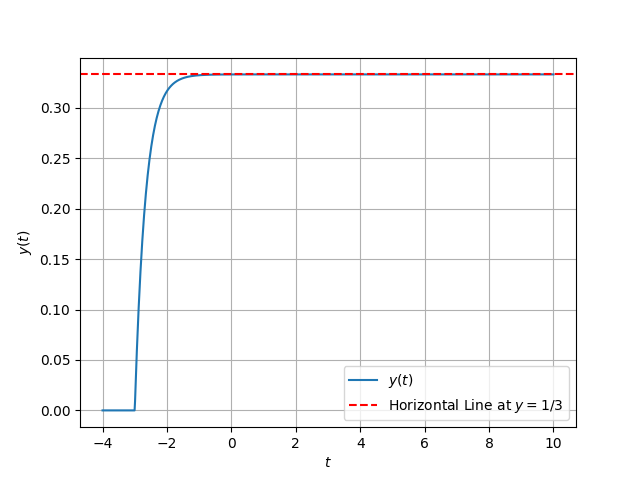
\includegraphics[width=0.8\columnwidth]{2021/IN/43/figs/plot.png}
    \caption{plot of $y(t)$}
    \label{fig:gate202138fig}
\end{figure}
%\end{document}
